The excess transverse energy coming from pile-up jets is generally subtracted on
average from the signal energy, however, due to localized fluctuations in the
pile-up, some of it remains in the $\pt$ of the reconstructed jet. The \gls{jvf}
is a variable that uses information from the track associated to each jet to
identify the origin vertex of each jet and rejects it if not coming from a
hard-scatter vertex~\cite{JVF}. The JVF can be regarded as a measure of the
fraction of the jet momentum associated with a primary vertex and is defined as:
\begin{equation}
  \label{eq:77}
  \mathrm{JVF} = \frac{\sum_k p_\mathrm{\, T}^\mathrm{\, trk_k}
    (\mathrm{PV_0})}{\sum_l p_\mathrm{\, T}^\mathrm{\, trk_l} (\mathrm{PV_0}) +
    \sum_{n \geq l} \sum_k p_\mathrm{\, T}^\mathrm{\, trk_l} (\mathrm{PV_n})}
\end{equation}
where PV$_0$ is the hard scatter vertex and PV$_\mathrm{n}$ with
$\mathrm{n} \geq 1$ is any other pile--up PV in the same bunch crossing thus
$\sum_k p_\mathrm{\, T}^\mathrm{\, trk_k} (\mathrm{PV_0})$ is the scalar $\pt$
sum of the tracks associated with the jet and originating from the hard scatter
vertex while
$\sum_{n \geq l} \sum_k p_\mathrm{\, T}^\mathrm{\, trk_l} (\mathrm{PV_n})$ is
the scalar $\pt$ sum of the tracks associated with the pile--up vertexes.

Since the JVF denominator increases with the number of reconstructed PV, this
introduces a pile-up dependence on the number of PV when minimal JVF selections
are imposed in rejecting pile--up jets. To address this problem, two new
variables to separate between \gls{hs} and \gls{pu} jets are introduced:
$\mathrm{corrJVF}$ and $\mathrm{R_{pT}}$. The former is defined as:
\begin{equation}
  \label{eq:78}
  \mathrm{corrJVF} = \frac{\pt^{\mathrm{\, HS}}}{\pt^{\, \mathrm{HS}} +
    \pt^{\, \mathrm{PU, corr}}}
\end{equation}
where
$\pt^{\mathrm{\, HS}} = \sum_k p_\mathrm{\, T}^\mathrm{\, trk_k}
(\mathrm{PV_0})$
is the scalar sum of the $\pt$ of the tracks associated with the jet that comes
from the hard scatter vertex and
$\pt^{\, \mathrm{PU, corr}} = \sum_{n \geq l} \sum_k p_\mathrm{\, T}^\mathrm{\,
  trk_l} (\mathrm{PV_n}) / (k n_{\mathrm{trk}}^{\mathrm{PU}})$
is the scalar sum of the associated tracks originating from a pile-up
vertex. Since the average $\pt^{\mathrm{PU}}$ increases linearly with the number
of pile-up tracks, $n_{\mathrm{trk}}^{\mathrm{PU}}$, $\pt^{\mathrm{PU}}$ is
divided by $(kn_{\mathrm{trk}}^{\mathrm{PU}})$ where $k = 0.01$ is the slope of
the $\langle \pt^{\mathrm{PU}} \rangle$ dependence with
$n_{\mathrm{trk}}^{\mathrm{PU}}$~\cite{JVT}. The corrJVF corrects the
N$_\mathrm{PV}$ dependence in the JVF denominator.

Finally the quantity $\mathrm{R_{pT}}$ is defined for each jet as:
\begin{equation}
  \label{eq:79}
  \mathrm{R_{pT}} = \frac{\sum_k p_\mathrm{\, T}^\mathrm{\, trk_k}
    (\mathrm{PV_0})}{\pt^{\mathrm{jet}}}
\end{equation}
where $\pt^{\mathrm{jet}}$ is the fully calibrated jet $\pt$. This variable is
defined using tracks associated with the vertex, it is at first order
independent on the N$_{\mathrm{PV}}$~\cite{PileUpPerformance}.

The \gls{jvt} is constructed from the corrJVF and $\mathrm{R_{pT}}$ by forming a
two dimensional likelihood based on the k-nearest neighbor algorithm. Using the
JVT algorithm, the HS jet efficiency is stable within 1\% up to 35 interactions
per bunch crossing~\cite{JVT}. \cref{fig:jvt_jvf} shows the hard scatter jet
efficiency dependence as a function of the average number of interactions per
bunch crossing $\mu$ for a target signal efficiency of 95\%. It can be seen that
the JVT distribution, within statistical error, is flat and performs better than
JVF at high pile--up as expected.
\begin{figure}[!h]
  \centering
    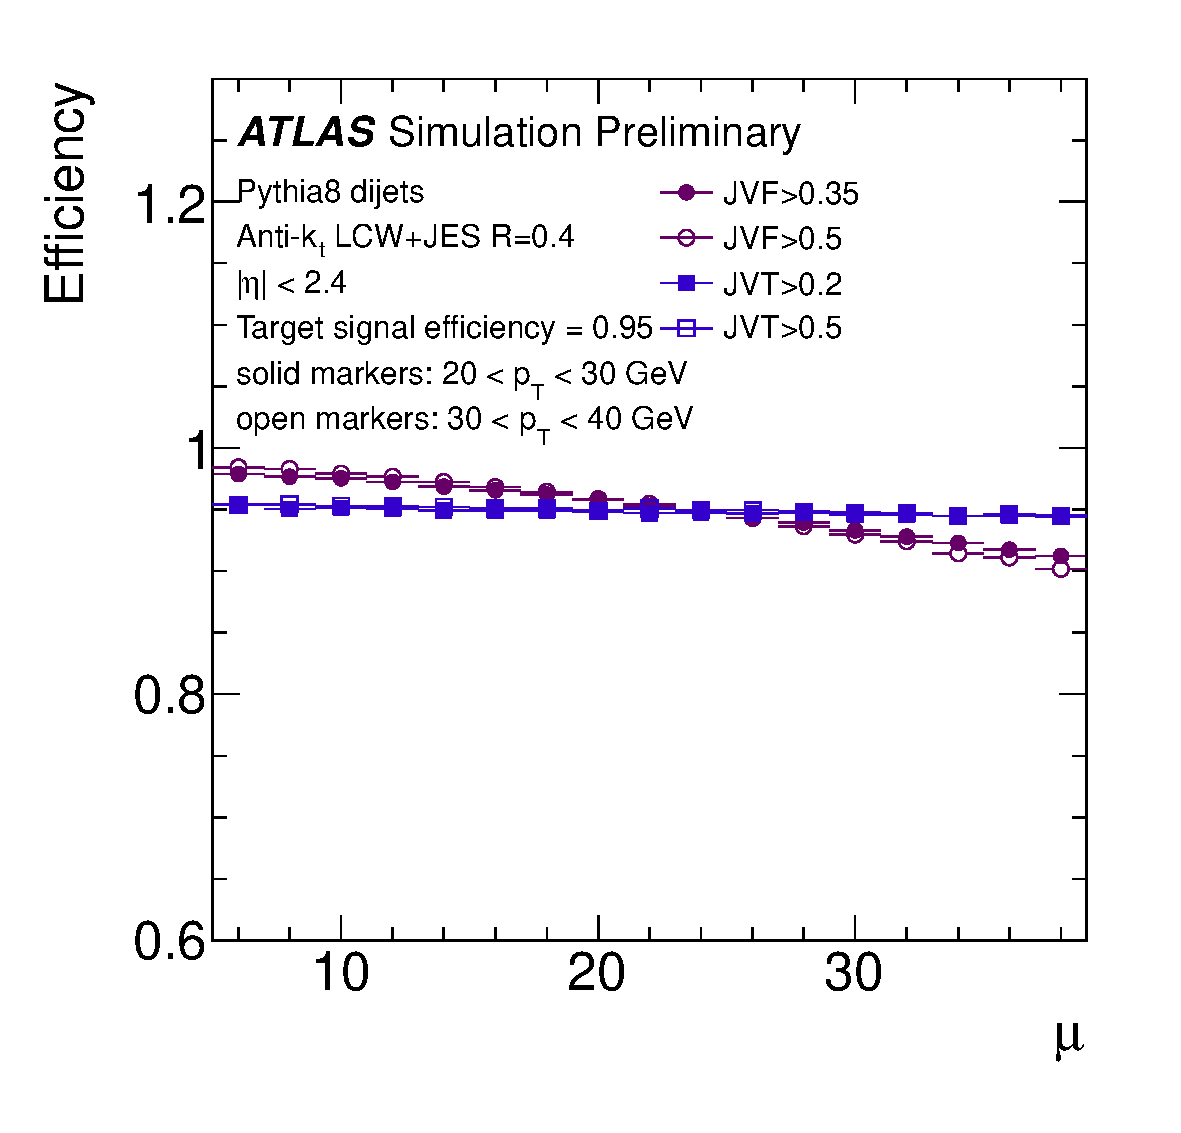
\includegraphics[width=.8\linewidth]{jvt_jvf}
    \caption{Dependence of the hard scatter jet efficiency as a function of the
      average number of interactions per bunch crossing $\nu$. The solid markers
    refers to jets with $20~<~\pt~<30$~GeV while the open markers to jets with
    $30~<~\pt~<40$~GeV. Fixed cuts on JVT (blue) and JVF (purple) are imposed
    such that the inclusive efficiency is 95\%~\cite{JVT}.}
    \label{fig:jvt_jvf}
\end{figure}
%%% Local Variables:
%%% mode: latex
%%% TeX-master: "../search_for_DM_LED_with_ATLAS"
%%% End:
